\documentclass[aspectratio=169]{beamer}
\geometry{paperwidth=160mm,paperheight=100mm}
\usepackage{beamerthemesidebar}
\usepackage{hyperref}
\usepackage{color}
\usepackage{multimedia}
\usepackage{colortbl}
\usepackage{amsmath}
\usepackage{empheq}
\usepackage{cancel}
\usepackage{amssymb}
\usepackage{amsfonts}
\usepackage{lipsum}
\usepackage{tcolorbox}
\usepackage{tabularx}
\usepackage{caption}
\usepackage{bm}

\setbeamersize{sidebar width right=0pt}
\setbeamertemplate{footline}[frame number]
%
\definecolor{orange}{RGB}{250,167,12}
\definecolor{yellow}{RGB}{246,250,12}
\definecolor{green}{RGB}{128,238,1}
\definecolor{black}{RGB}{0,0,0}
\definecolor{blue}{RGB}{0,0,255}
\definecolor{red}{RGB}{255,0,0}
\definecolor{sepia}{RGB}{94,38,18}
\newcommand{\ve}[1]{{\rm\bf {#1}}}
\newcommand{\q}[1]{\textcolor{blue}{#1}}
\newcommand{\blue}[1]{\textcolor{blue}{#1}}
\newcommand{\sepia}[1]{\textcolor{sepia}{#1}}
\newcommand{\red}[1]{\textcolor{red}{#1}}
\newcommand{\green}[1]{\textcolor{green}{#1}}
\newcommand{\yellow}[1]{\textcolor{yellow}{#1}}
\newcommand{\orange}[1]{\textcolor{orange}{#1}}
\definecolor{burlywood}{RGB}{255,211,155}
\definecolor{chocolate}{RGB}{255,127,36}
\definecolor{tan}{RGB}{210,180,140}
%
\def\onethird{{\textstyle{1\over3}}}
\def\twothirds{{\textstyle{2\over3}}}
\def\fourthirds{{\textstyle{4\over3}}}
\def\onehalf{{\textstyle{1\over2}}}
\def\threehalfs{{\textstyle{3\over2}}}
%
\newcommand{\pd}{\partial}
\newcommand{\aMLT}{\alpha_{\rm MLT}}
\newcommand{\Fconv}{F_{\rm conv}}
\newcommand{\Frad}{F_{\rm rad}}
\newcommand{\Ftot}{F_{\rm tot}}
\newcommand{\Hp}{H_p}
\newcommand{\prad}{p_{\rm rad}}
\newcommand{\pgas}{p_{\rm gas}}
\newcommand{\TTc}{T_{\rm c}}
\newcommand{\rhoc}{\rho_{\rm c}}
\newcommand{\Teff}{T_{\rm eff}}
\newcommand{\Fstar}{F_\star}
\newcommand{\pstar}{p_\star}
\newcommand{\Pstar}{P_\star}
\newcommand{\Rstar}{R_\star}
\newcommand{\rhostar}{\rho_\star}
\newcommand{\Tstar}{T_\star}
%
\title{Theoretical Astrophysics I: Physics of Sun and Stars\\
Lecture 9: Stellar Atmospheres}
\author{\texorpdfstring{\sepia{Petri K\"{a}pyl\"{a} Ivan Mili\'{c}}\newline\blue{\url{pkapyla, milic@leibniz-kis.de}}}{}}
\institute{Institut f\"ur Sonnenphysik - KIS, Freiburg}
\date{\today}
%
\begin{document}
\frame{\titlepage}


\section{Recap and intro}
%
\frame{
\frametitle{Recap}
\begin{itemize}
\item So far we have dealt with interiors of the stars - these contain an absolute majority of stellar material. 
\item We studied the equations that govern stellar structure and the evolution and solved them in more or less detail to understand how the stars look into the inside and how they evolve on the HR diagram. 
\item None of these processes were \textbf{directly} observable. The only observable quantity we talked about was the stellar luminosity ($L$). 
\item Now we are going to talk about the structures that we can observe - stellar atmospheres, and their observational signatures - stellar spectra. 
\end{itemize}
}
%
%
\frame{
\frametitle{Why study stellar atmospheres?}
\begin{minipage}{0.54\linewidth}
\begin{itemize}
\item Stellar atmosphere is the miniscule part on the very right of this diagram. 
\item How can it be important? (Salpeter once asked the same question)
\item First: Stellar atmosphere is the only part we can observe: insight into what is going on inside. 
\item Second: It can influence the evolution of the star, at certain evolution stages atmospheres can be huge and influence the rest. 
\item Third: There is a lot of interesting physics going on (especially the case for the Sun, talk next week!)
\end{itemize}
\end{minipage}
\begin{minipage}{0.45\linewidth}
\begin{figure}
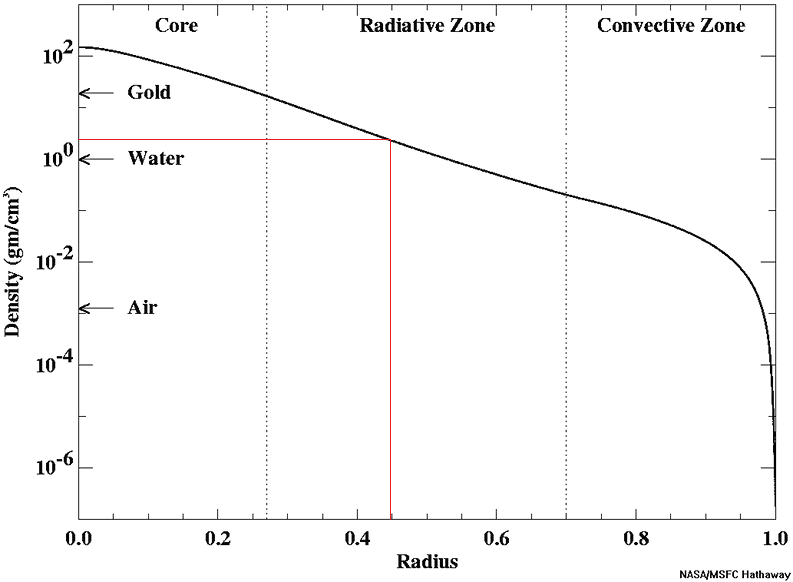
\includegraphics[width=6cm]{figures/solar_density.png}
\caption*{Credits: NASA/MSFC Hathaway}
\end{figure}
\end{minipage}
}
%
%
\frame{
\frametitle{Differences between stellar atmospheres and stellar interiors}
\begin{minipage}{0.495\linewidth}
Interior
\begin{itemize}
\item $T = 10^5 - 10^7$\,K
\item $\rho = 10^{1} - 10^{5} {\rm kg / m^3}$
\item Completely ionized 
\item Ideal gas
\item LTE 
\end{itemize}
\end{minipage}
\begin{minipage}{0.495\linewidth}
Atmospheres
\begin{itemize}
\item $T = 10^4 - 10^5$\,K
\item $\rho = 10^{-1} - 10^{-8} {\rm kg / m^3}$
\item Neutral, partially ionized, totally ionized - depending on the layer and species
\item Ideal gas
\item Photosphere in LTE, chromosphere and up in NLTE, but some things are tricky (e.g. photoionization)
\end{itemize}
\end{minipage}

}
%
%
\frame{
\frametitle{Sketch of the atmosphere}
\begin{minipage}{0.495\linewidth}
\begin{itemize}
  \item Atmospheres of main sequence stars are typically very thin: plane-parallel approximation is valid. 
  \item The transport of energy goes from convective to radiative, and then the energy leaves the star. 
  \item Radiative equilibrium is often used: $H=const$.
  \item To understand the observational signatures of the atmosphere we need to:
  \item i) mathematically describe propagation of radiation;
  \item ii) take into account appropriate physical processes that contribute to opacity and emissivity;
\end{itemize}
\end{minipage}
\begin{minipage}{0.495\linewidth}
\begin{figure}
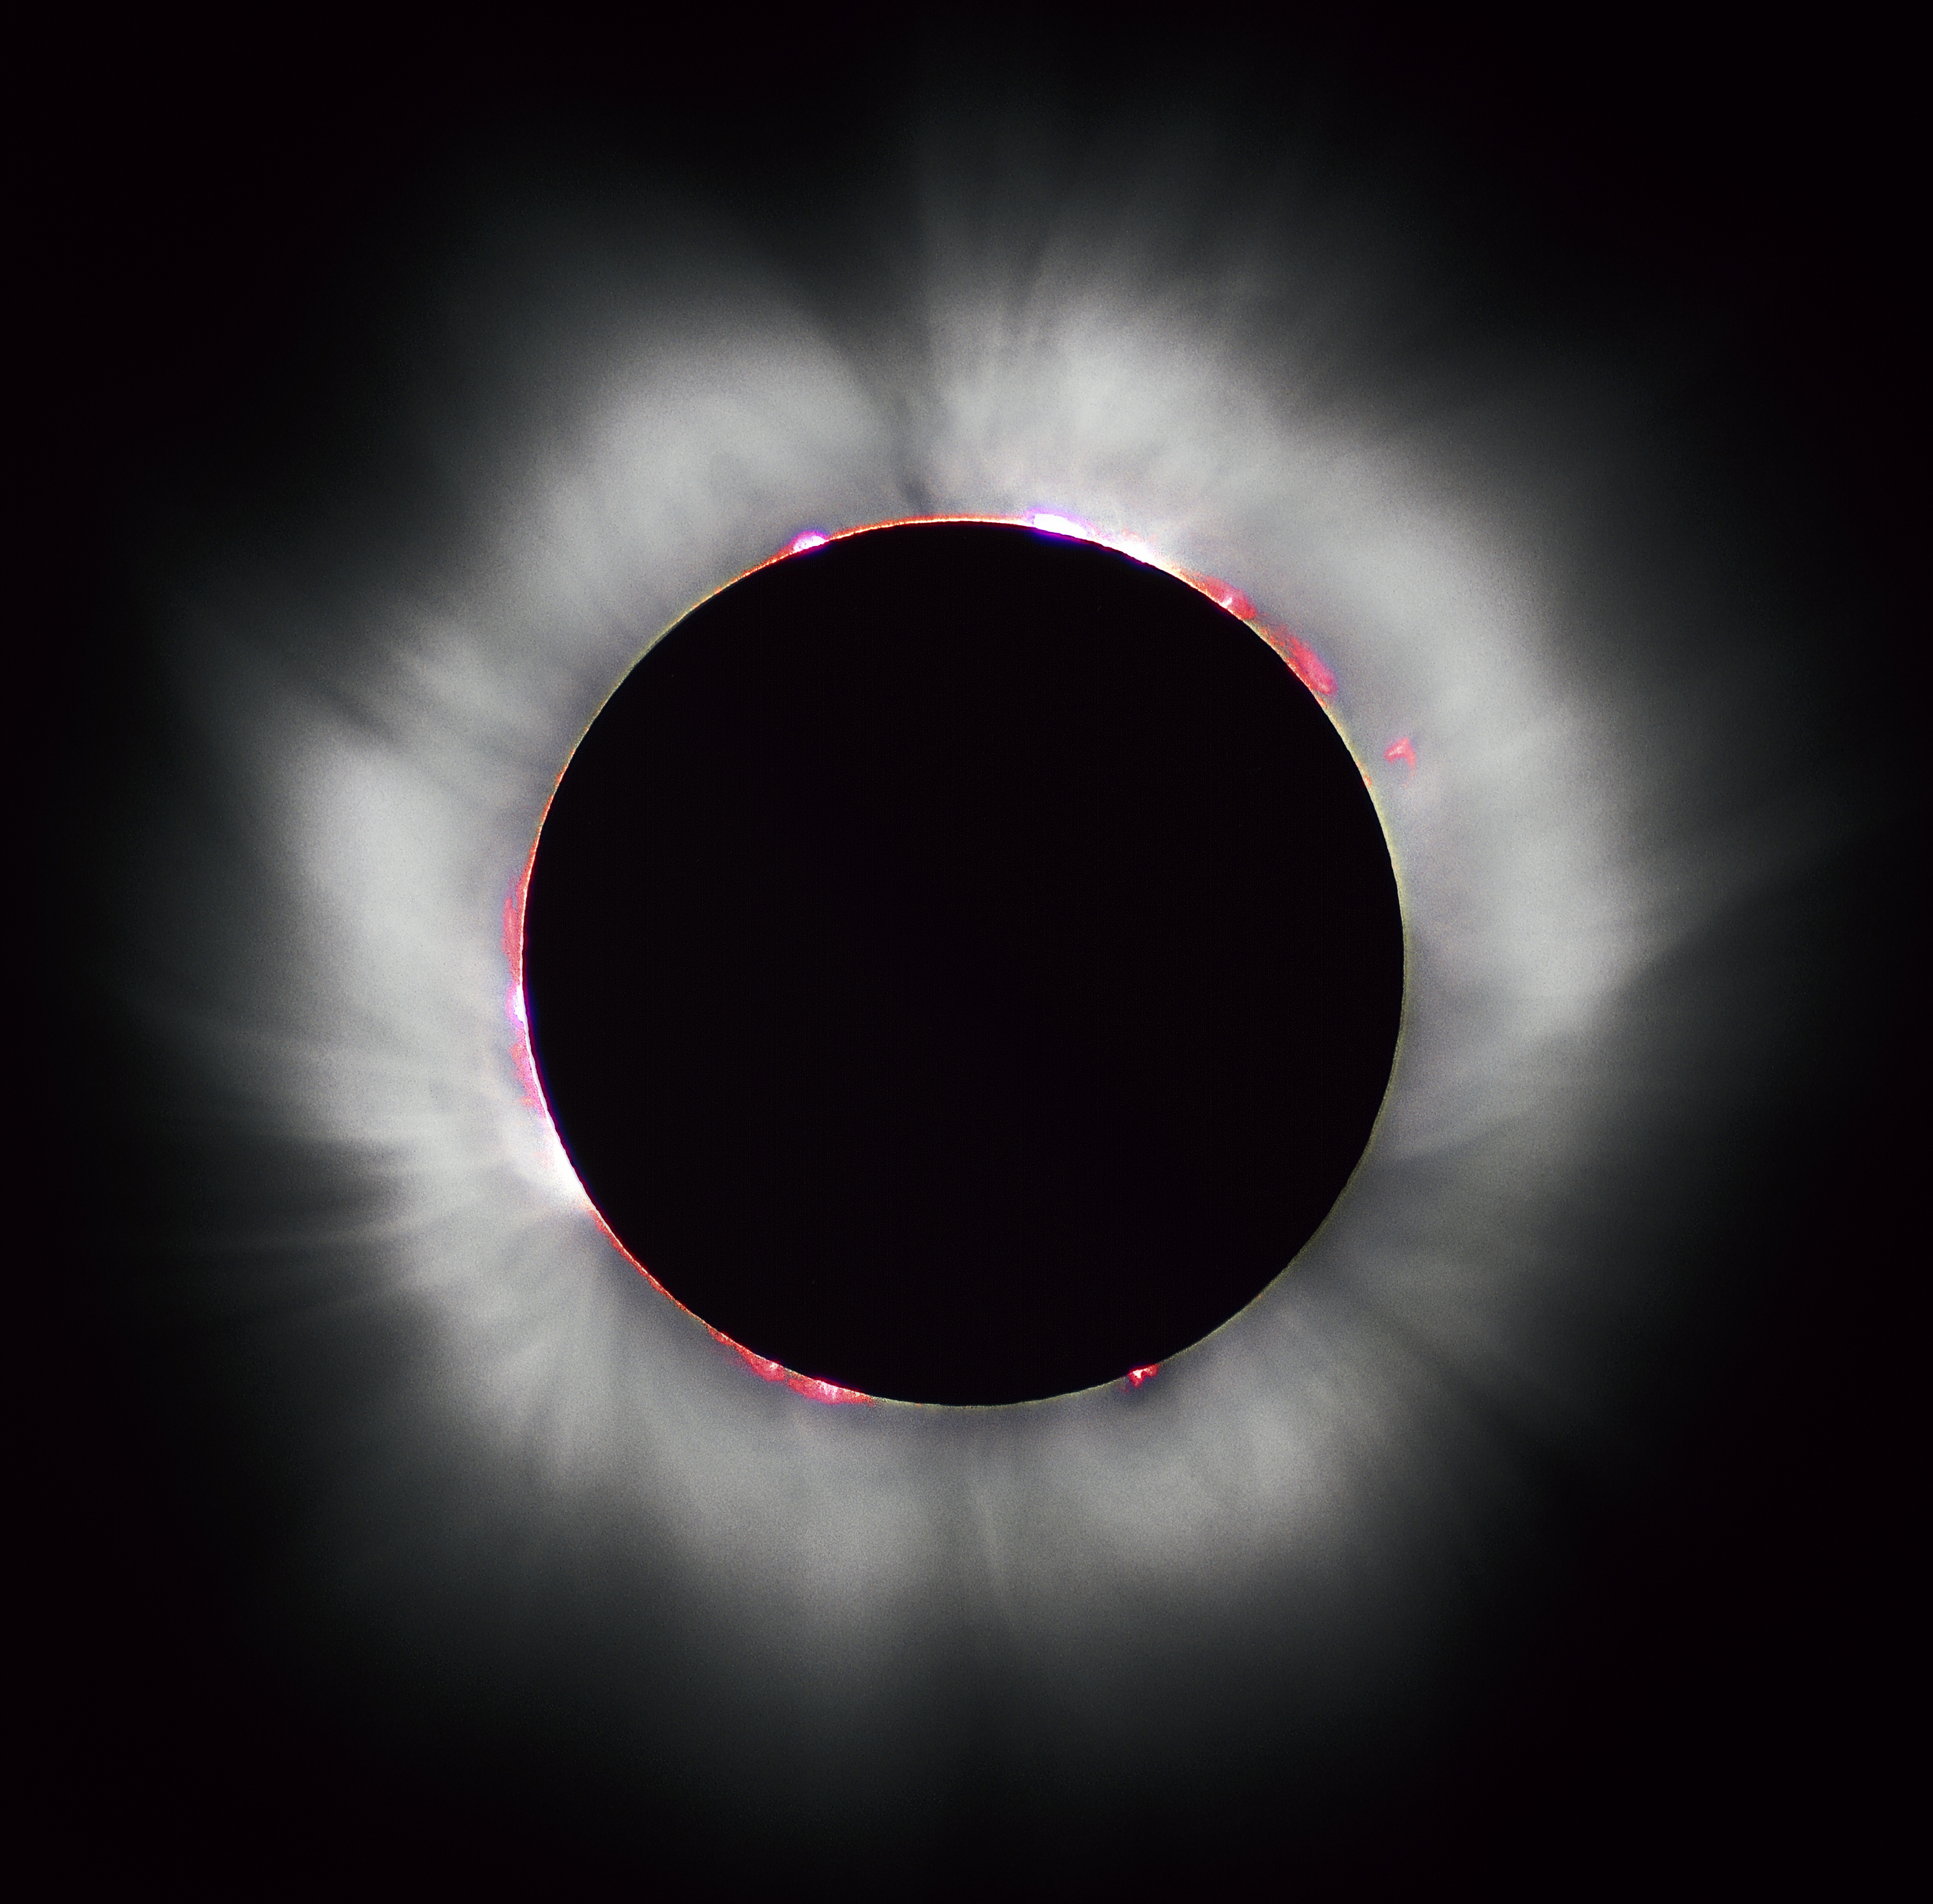
\includegraphics[width=6cm]{figures/Solar_eclipse_1999_4.jpg}
\caption*{Credits: Wikipedia}
\end{figure}
\end{minipage}

}
%
%
\frame{
\frametitle{Spectral classses}
\begin{minipage}{0.44\linewidth}
\begin{itemize}
  \item One of the main features we want to understand are the differences between the different spectral classes.
  \item For a while - people thought that these differences are due to different chemical composition. 
  \item But it turns out stellar spectra are \textbf{extremely} sensitive to the temperature and the pressure.
  \item Today, we will try to explain that.
\end{itemize}
\end{minipage}
\begin{minipage}{0.55\linewidth}
\begin{figure}
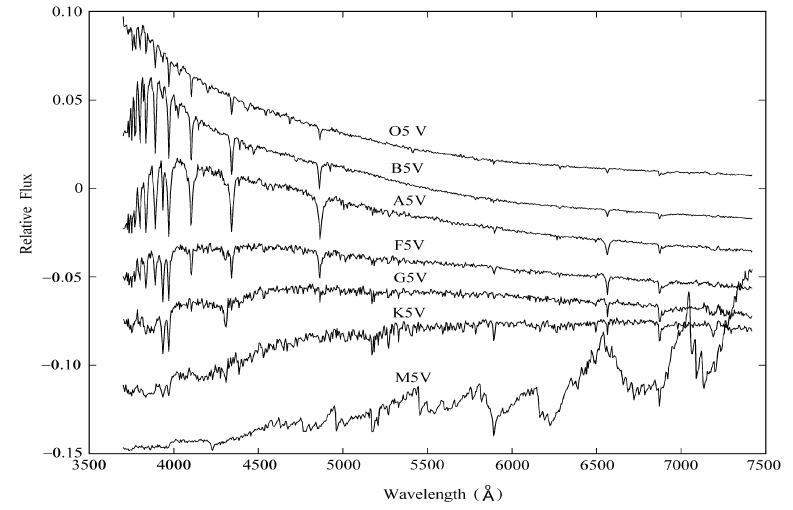
\includegraphics[width=7.5cm]{figures/stel_spec.png}
\caption*{Credits: Wikipedia}
\end{figure}
\end{minipage}

}
\section{Radiative Transfer Equation}
%
%
\frame{
\frametitle{Specific monochromatic intensity}
\begin{minipage}{0.5\linewidth}
\begin{itemize}
\item We need to treat wavelength and angular dependence of the radiation field
\item Intensity: energy transported through given area in given time per given solid angle and frequency/wavelength bin (note the deprojection factor $\cos \theta$).
\begin{equation}
I_\nu = \frac{dE}{dS\,dt\,d\Omega\,d\nu\,\cos \theta}
\end{equation}
\item Going to number of photons:
\begin{equation}
n(\theta,\phi\,\nu) = \frac{I_\nu}{c\,h\nu}
\end{equation}
\end{itemize}
\end{minipage}
\begin{minipage}{0.49\linewidth}
\begin{figure}
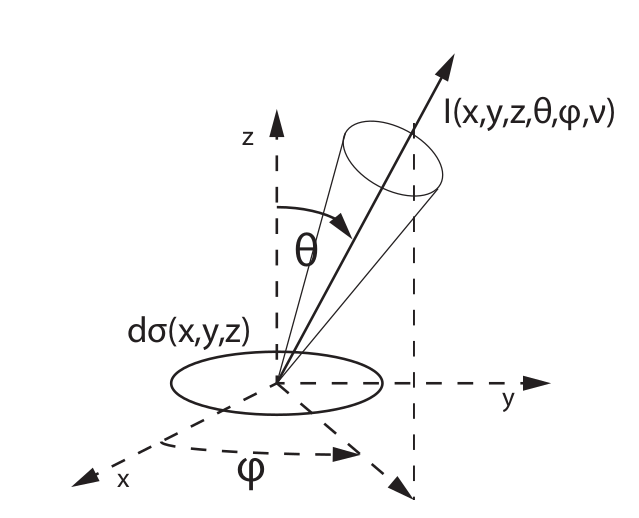
\includegraphics[width=6.0cm]{figures/spec_int.png}
\caption*{Credits: IM thesis (2014, University of Belgrade)}
\end{figure}
\end{minipage}
}
%
\frame{
\frametitle{Radiative Transfer Equation (RTE)}
\begin{minipage}{0.5\linewidth}
\begin{itemize}
\item This formulation is (more or less) due to Kirchhoff. The change of intensity ``along-the-ray'' over a distance $ds$ is:
\begin{equation}
dI_\nu = \eta_\nu ds - \chi_\nu I_\nu ds 
\end{equation} 
\item The terms of the right represent emission and \textbf{total} absorption (both true absorption and scattering) per unit volume.
\end{itemize}
\end{minipage}
\begin{minipage}{0.49\linewidth}
\begin{figure}
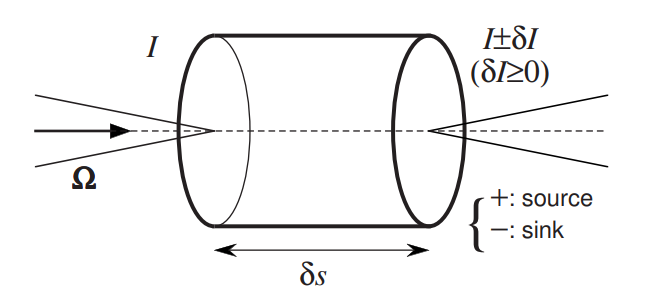
\includegraphics[width=6cm]{figures/rte_1.png}
\caption*{Credit: Anthony B. Davis and Yuri Knyazikhin}
\end{figure}
\end{minipage}
}
%
%
\frame{
\frametitle{Radiative Transfer Equation}
\begin{minipage}{0.55\linewidth}
\begin{itemize}
\item Now, it makes sense that the absorption and emission properties of the medium depend on:
\item Amount of matter capable of absorbing/emitting
\item The inherent properties of the matter at the given temperature ($T$ is very important!)
\item So we define:
\begin{align}
\kappa_\nu = \chi_\nu / \rho \\
j_\nu = \eta_\nu / \rho
\end{align}
\item So our equation becomes:
\begin{equation}
\frac{1}{\rho} \frac{dI_\nu}{ds} = -\kappa_\nu I_\nu + j_\nu
\end{equation}
\end{itemize}
\end{minipage}
\begin{minipage}{0.44\linewidth}
\begin{figure}
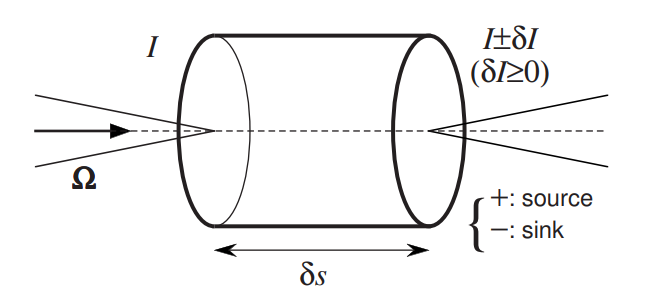
\includegraphics[width=6cm]{figures/rte_1.png}
\caption*{Credit: Anthony B. Davis and Yuri Knyazikhin}
\end{figure}
\end{minipage}
}
%
\frame{
\frametitle{Optical depth and Source function}
\begin{minipage}{0.55\linewidth}
\begin{itemize}
\item We often do the following:
\begin{equation}
\frac{dI_\nu}{-\rho \kappa_\nu ds} = I_\nu - j_\nu / \kappa_\nu
\end{equation}
\item And we get:
\begin{equation}
\frac{dI_\nu}{-\rho \kappa_\nu ds} = I_\nu - j_\nu / (\rho \kappa_\nu)
\end{equation}

\begin{align}
\kappa_\nu = \chi_\nu / \rho; \,j_\nu = \eta_\nu / \rho
\end{align}
\item So our equation becomes:
\begin{equation}
\frac{dI_\nu}{d\tau_\nu} = I_\nu - S_\nu
\end{equation}
\end{itemize}
\end{minipage}
\begin{minipage}{0.44\linewidth}
\begin{figure}
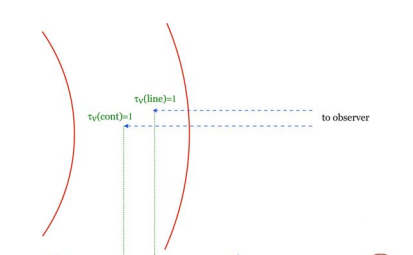
\includegraphics[width=6cm]{figures/tau.png}
\caption*{Credit: Rolf Kudritzki}
\end{figure}
\end{minipage}
}
%
\section{Solving RTE}
%
\frame{
\frametitle{Optical depth and Source function}
\begin{minipage}{0.55\linewidth}
\begin{equation}
\frac{dI_\nu}{d\tau_\nu} = I_\nu - S_\nu
\end{equation}
\begin{itemize}
\item Solving this equation if everything is known is relatively straightforward:
\begin{equation}
dI_\nu = I_\nu^0 e^{-\tau_\nu} + \int_0^{\tau_\nu} S(t) e^{-t} dt
\end{equation}
\item Here $t$ is the dummy variable for frequency dependent optical depth.
\item \textbf{Please note that the optical depth depends on the frequency!} \q{Discuss!}
\end{itemize}
\end{minipage}
\begin{minipage}{0.44\linewidth}
\begin{figure}
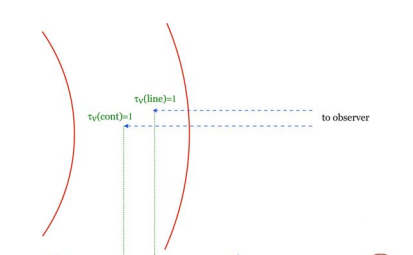
\includegraphics[width=6cm]{figures/tau.png}
\caption*{Credit: Rolf Kudritzki}
\end{figure}
\end{minipage}
}
%
%
\frame{
\frametitle{Optical depth}
\begin{minipage}{0.55\linewidth}
\begin{equation}
\tau_\nu = \int -\rho \kappa_\nu ds
\end{equation}
\begin{itemize}
\item As the absorption and scattering properties (opacity) of the medium depend on the wavelength, so does the optical depth.
\item Now, why does the opacity depend on the wavelength? \q{Discuss!}
\item Right: opacity due to bound-free absorption of neutral hydrogen atom.
\end{itemize}
\end{minipage}
\begin{minipage}{0.44\linewidth}
\begin{figure}
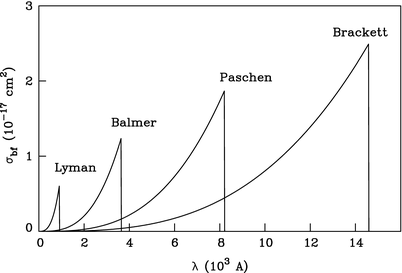
\includegraphics[width=6cm]{figures/hbf.png}
\caption*{Credit: Rolf Kudritzki}
\end{figure}
\end{minipage}
}
%
%
\frame{
\frametitle{Constant source function}
\begin{minipage}{0.55\linewidth}
\begin{equation}
dI_\nu = I_\nu^0 e^{-\tau_\nu} + \int_0^{\tau_\nu} S(t) e^{-t} dt
\end{equation}
\begin{itemize}
\item For a slab of constant source function, we get:
\begin{equation}
dI_\nu = I_\nu^0 e^{-\tau_\nu} + S_\nu (1-e^{-\tau_\nu})
\end{equation}
\item Depending on the $\tau_\nu$ we can get either dominant contribution of the background radiation, or the slab. 
\item \q{Discuss the image on the right (solar atmosphere imaged at two different wavelengths)}
\end{itemize}
\end{minipage}
\begin{minipage}{0.44\linewidth}
\begin{figure}
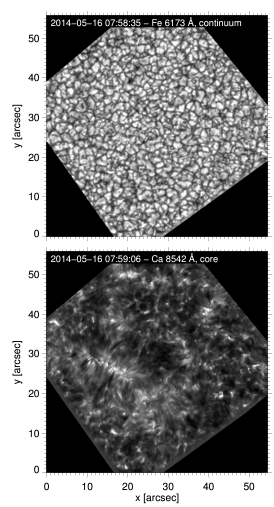
\includegraphics[width=4.5cm]{figures/gosic.png}
\caption*{Credit: Gosic et al., 2018}
\end{figure}
\end{minipage}
}
%
%
\frame{
\frametitle{Constant source function}
\begin{minipage}{0.55\linewidth}
\begin{equation}
dI_\nu = I_\nu^0 e^{-\tau_\nu} + S_\nu (1-e^{-\tau_\nu})
\end{equation}
\begin{itemize}
\item We can now frame this differently:
\item If we somehow \textbf{know} that, at a wavelength the medium is \textbf{optical thick}, we know we are seeing that medium.
\item If it is \textbf{transparent}, we know we are seeing the light below. 
\item So we can use different wavelengths to probe different regions. 
\item But, sometimes differences between $S$ and 
\end{itemize}
\end{minipage}
\begin{minipage}{0.44\linewidth}
\begin{figure}
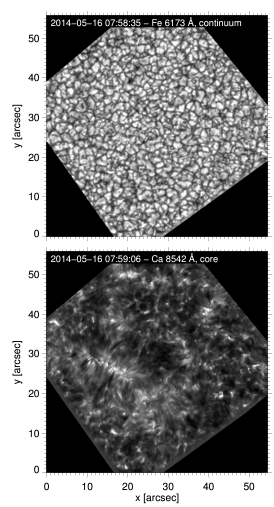
\includegraphics[width=4.5cm]{figures/gosic.png}
\caption*{Credit: Gosic et al., 2018}
\end{figure}
\end{minipage}
}
%
%
\frame{
\frametitle{Linear source function with depth}
\begin{itemize}
  \item A very often used assumption in the atmosphere modeling is the so called, Milne-Eddington model, it assumes that, at some \emph{referent} wavelength, we have:
\begin{equation}
S_\nu = a + b \tau_r
\end{equation}
\item where $\tau_r$ is the optical depth at that referent wavelength.
\item We define $r_\nu$, which is the ratio of opacities at other frequencies (wavelengths) to the referent one. 
\item Additionally, we will assume that $S_\nu = B_\nu$ (LTE), and that $\tau_\nu >> 1$, we get:
\begin{equation}
dI_\nu = \int_0^{\infty} (a + b \tau_r) e^{-\tau_r r_\nu} d \tau_r r_\nu
\end{equation}
\item That yields (\q{blackboard!}):
\begin{equation}
dI_\nu = a + b / r_\nu
\end{equation}

\end{itemize}
}
%
%
\frame{
\frametitle{Linear source function with depth}
\begin{minipage}{0.5\linewidth}
\begin{equation}
dI_\nu = a + b / r_\nu
\end{equation}
\begin{itemize}
\item It is reasonable to assume that $S$ increases inward in the solar atmosphere (because $T$ increases), so $a$ and $b$ are positive.
\item For more opaque regions we will get less intensity.
\item Wow - not really insightful after all!
\item Extremely important: we also understood that a \textbf{gradient} of temperature in the atmosphere is necessary!
\end{itemize}
\end{minipage}
\begin{minipage}{0.49\linewidth}
\begin{figure}
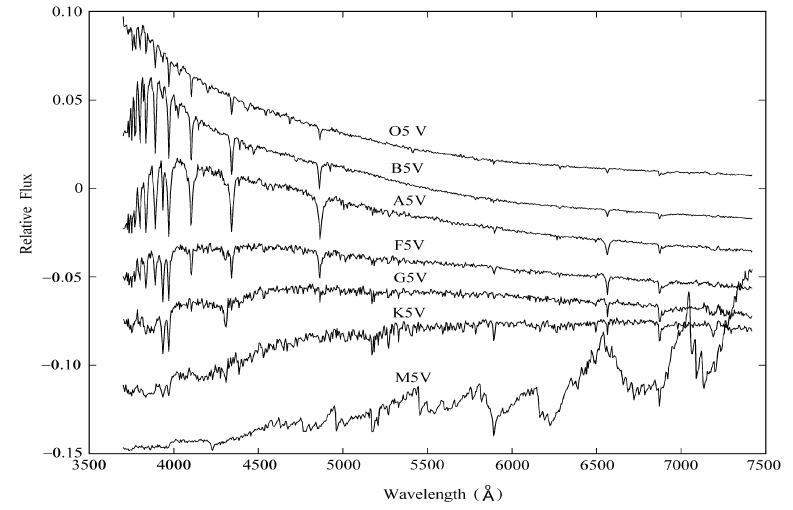
\includegraphics[width=6.7cm]{figures/stel_spec.png}
\caption*{Credits: Wikipedia}
\end{figure}
\end{minipage}
}
%
\section{Milne problem}
%
\frame{
\frametitle{Why the Milne-Eddington approximation}
\begin{itemize}
  \item Why choose linear, why not quadratic? Why not some other functional dependence?
  \item Beginning of XX century, Eddington, Milne, Schwarzschild and company were trying to solve the structure of the stellar atmosphere in radiative equilibrium. 
  \item Given the outgoing specific flux ($H$), find the structure of the atmosphere. 
  \item Radiative equilibrium (your hw):
  \begin{equation}
  \int_0^{\infty} \kappa_\nu J_\nu d_\nu = \int_0^{\infty} \kappa_\nu S_\nu d_\nu
  \end{equation}
  \item Was simplified, by assuming that there is some mean $\overline{\kappa}$ (gray atmosphere), so that:
  \begin{equation}
  J = S
  \end{equation}
  \item Furthermore, it was reasonable to assume LTE, so that $S=B=\sigma T^4 = J$.
  \item This is a direct connection between the radiation and the temperature.
  \item But how to find $J(z)$, or better to say $J(\tau)$?
\end{itemize}
}
%
%
\frame{
\frametitle{Milne problem}
\begin{itemize}
  \item But how to find $J(z)$, or better to say $J(\tau)$? We did not use RTE yet. Define that optical depth goes in the negative z direction: 
  \begin{equation}
  \mu\frac{dI}{d\tau} = I - S = I - J
  \end{equation}
  \item Integrate this over $d \mu$ and $\mu d \mu$. \q{We will need the blackboard here!}
  \item You should get...
\end{itemize}
}
%
\frame{
\frametitle{Milne problem}
\begin{itemize}
  \item But how to find $J(z)$, or better to say $J(\tau)$? We did not use RTE yet. Define that optical depth goes in the negative z direction: 
  \begin{equation}
  \mu\frac{dI}{d\tau} = I - S = I - J
  \end{equation}
  \item Integrate this over $d \mu$ and $\mu d \mu$. \q{We will need the blackboard here!}
  \item You should have gotten:
  \begin{equation}
  \frac{dH}{d\tau} = 0
  \end{equation}
  \item and:
  \begin{equation}
  \frac{dK}{d\tau} = H
  \end{equation}
  \item This is where Eddington made an approximation to try and ``close'' the system, he assumed that $K=J/3$, and thus: 
  \begin{equation}
  J = 3H \tau + {\rm const} = a \tau + b
  \end{equation}
  \item This can later be pursued further to infer the temperature structure of a gray atmosphere, but we will not go there.
  

\end{itemize}
}
%
%
\frame{
\frametitle{Linear source function with depth}
\begin{minipage}{0.5\linewidth}
\begin{equation}
dI_\nu = a + b / r_\nu
\end{equation}
\begin{itemize}
\item It is reasonable to assume that $S$ increases inward in the solar atmosphere (because $T$ increases), so $a$ and $b$ are positive.
\item For more opaque regions we will get less intensity.
\item We ``solved'' mathematical part. Now is time for physics, because...
\item What we still don't understand is why the opacity varies with the wavelength.
\end{itemize}
\end{minipage}
\begin{minipage}{0.49\linewidth}
\begin{figure}
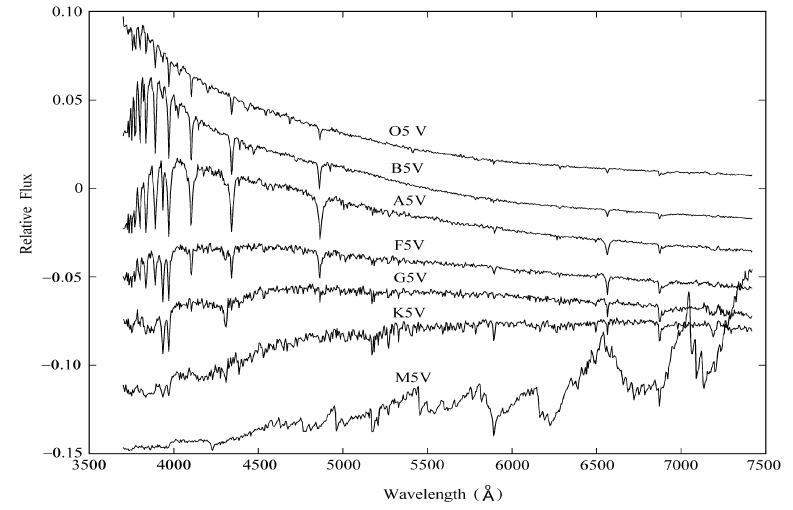
\includegraphics[width=6.7cm]{figures/stel_spec.png}
\caption*{Credits: Wikipedia}
\end{figure}
\end{minipage}
}
%
\section{Processes that contribute to opacity}
% 
\frame{
\frametitle{Opacity sources}
\begin{itemize}
\item Reminder, we only talk about opacity ($\kappa_\nu$) because $j_\nu = B_\nu \kappa_\nu$!
\item Important sources are:
\item Bound-free transitions (photoionization)
\item Free-free processes (inverse bremsstrahlung) - not important at low temperatures and optical wavelengths
\item Bound-bound processes (spectral lines - very diagnostically important!) \q{Discuss!}
\item Thomson and Rayleigh scattering. 
\item \textbf{Bound-free and free-free emission of $H-$ (very important for colder stars).}
\end{itemize}
}
%
%
\frame{
\frametitle{Bound-free opacity}
\begin{minipage}{0.55\linewidth}
\begin{itemize}
\item This is, in fact, photoionization. The energy of the photon needs to be larger than the binding energy of the electron:
\begin{equation}
h\nu > E_{ion}
\end{equation}
\item Higher levels are easier to ionize, so if we have more excited atoms, opacity at lower energies/ higher wavelengths is higher. \q{Talk about this for a while}.
\item For example, for hydrogen: $E_{ion} = 13.6{\rm eV} / i^2$, where $i$ is the principal quantum number of the level.
\begin{equation}
\rho \kappa_\nu^{bf} = \sum_i n_i \sigma_i
\end{equation}
\item where I denoted the cross-section with $\sigma$.
\end{itemize}
\end{minipage}
\begin{minipage}{0.44\linewidth}
\begin{figure}
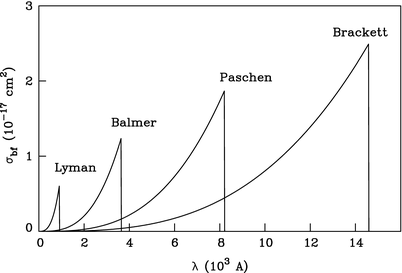
\includegraphics[width=6cm]{figures/hbf.png}
\end{figure}
\end{minipage}
}
%
%
\frame{
\frametitle{Bound-free opacity}
\begin{minipage}{0.55\linewidth}
\begin{itemize}
\item \q{What levels need to be populated so that hydrogen contributes to the opacity in the visible wavelengths?}
\item The Boltzman equation governs the excitations as: 
\begin{equation}
n_i = n_H \frac{g_i e^{-E_i / kT}}{Z_H}
\end{equation}
\item here $g_i$ is called \textbf{statistical weight} and $Z$ is the \textbf{partition function}.
But, we also need the concentration of the neutral hydrogen:
\begin{equation}
\frac{n_{H+} n_e}{n_H} = \frac{1}{\Lambda^3} e^{-E_{ion}/kT} 
\end{equation}
How does $n_{H}$ vary with temperature?
\end{itemize}
\end{minipage}
\begin{minipage}{0.44\linewidth}
\begin{figure}
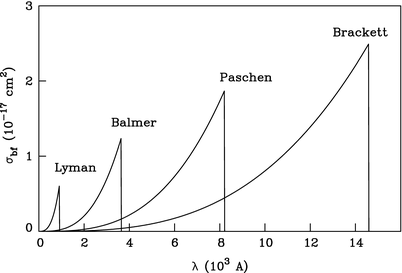
\includegraphics[width=6cm]{figures/hbf.png}
\end{figure}
\end{minipage}
}
% 
%
\frame{
\frametitle{Opacity in different physical conditions}
\begin{minipage}{0.55\linewidth}
\begin{itemize}
\item For low temperatures, hydrogen is neutral, but not excited.
\item For very high temperatures, hydrogen is ionized and cannot absorb in bound-free processes. 
\item The temperature where the ``optimum'' amount of absorption happens is around 10\,kK. 
\item Right: The variation of absorption coefficient with different contributions. Note the $H-$. (From Gray, 1992)
\end{itemize}
\end{minipage}
\begin{minipage}{0.44\linewidth}
\begin{figure}
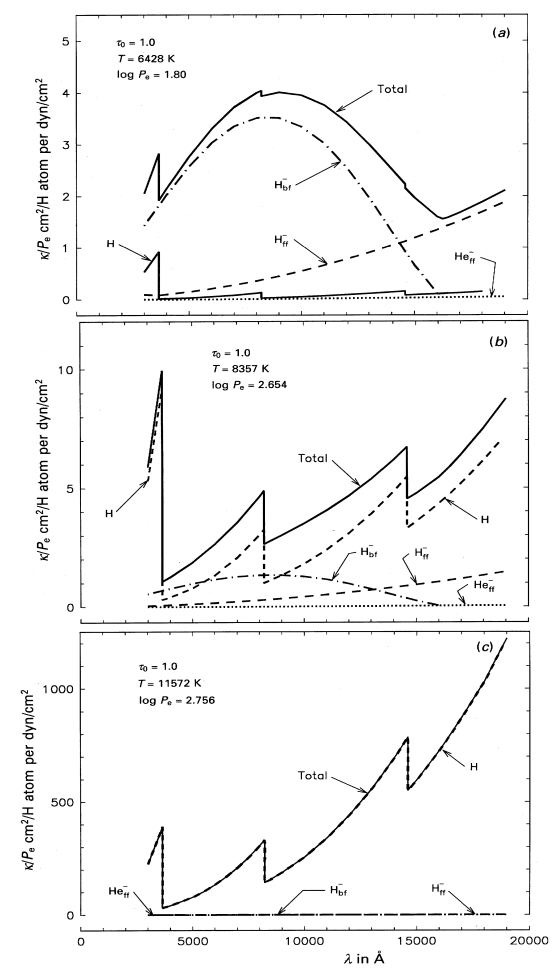
\includegraphics[width=5cm]{figures/grayop.png}
\end{figure}
\end{minipage}
}
% 
\frame{
\frametitle{Opacity due to negative ion of hydrogen}
\begin{minipage}{0.55\linewidth}
\begin{itemize}
\item Negative ion of hydrogen is a neutral hydrogen that captured an additional electron.
\item It is very easy to ionize, only 0.75\,eV is needed. (Maximum )
\item The temperature where the ``optimum'' amount of absorption happens is around 10\,kK. 
\item Right: The variation of absorption coefficient with different contributions. Note the $H-$. (From Gray, 1992)
\item \q{Time permitting- compare the number density of negative ion of hydrogen and neutral hydrogen excited to $i=3$, for solar photospheric conditions}
\end{itemize}
\end{minipage}
\begin{minipage}{0.44\linewidth}
\begin{figure}
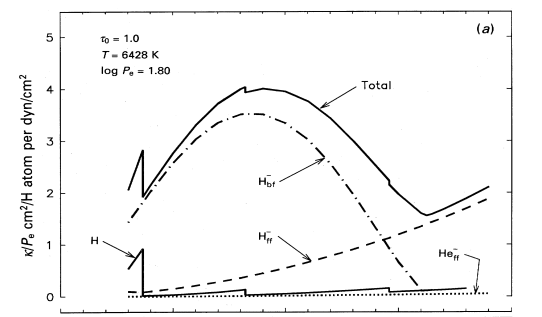
\includegraphics[width=6.5cm]{figures/hminus.png}
\end{figure}
\end{minipage}
}
% 
%
\frame{
\frametitle{Now we should understand this plot!}
\begin{figure}
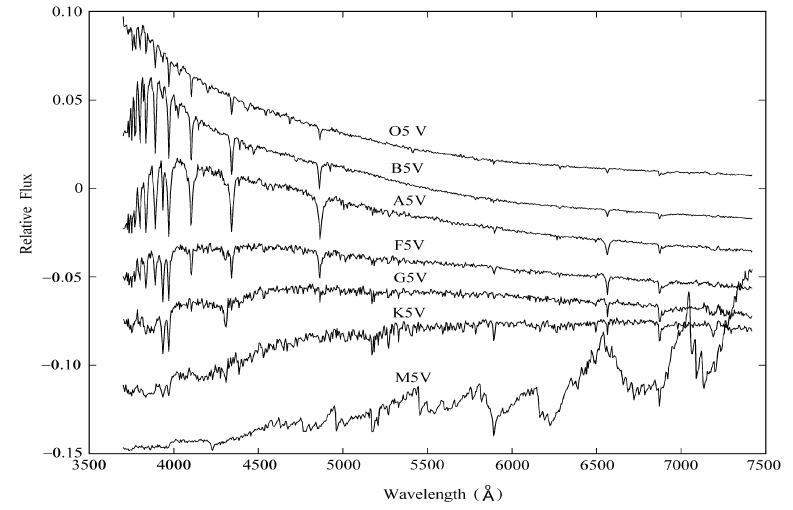
\includegraphics[width=11cm]{figures/stel_spec.png}
\caption*{Credits: Wikipedia}
\end{figure}
}
%
\section{Spectral lines}
%
\frame{
\frametitle{What other features can you see here?}
Spectral lines: features in the solar spectra that are result of \textbf{bound-bound} processes.
\begin{figure}
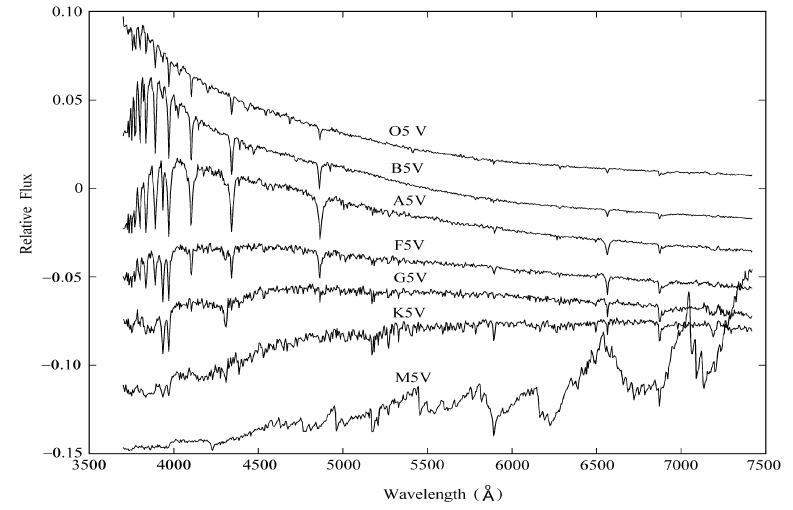
\includegraphics[width=8cm]{figures/stel_spec.png}
\caption*{Credits: Wikipedia}
\end{figure}
}
%
%
\frame{
\frametitle{Spectral lines in one slide}
\begin{minipage}{0.55\textwidth}
\begin{itemize}
\item Spectral lines can have extremely high opacity (and emissivity), but only over a very small range of wavelengths. 
\item To resolve spectral lines we need observations of high spectral resolution. 
\item We can write the absorption coefficient ($\chi_nu = \rho \kappa_\nu$) in a spectral line as:
\begin{equation}
\chi_\nu = n_i \sigma_0^{\rm line} \phi_\lambda
\end{equation}
\item Here $\sigma_0^{\rm line}$ is the so called line center absorption cross-section, which can be very high.
\item $\phi_\lambda$ is the line absorption profile, which goes from one in the line center to zero in the wings. 
\end{itemize}
\end{minipage}
\begin{minipage}{0.44\linewidth}
\begin{figure}
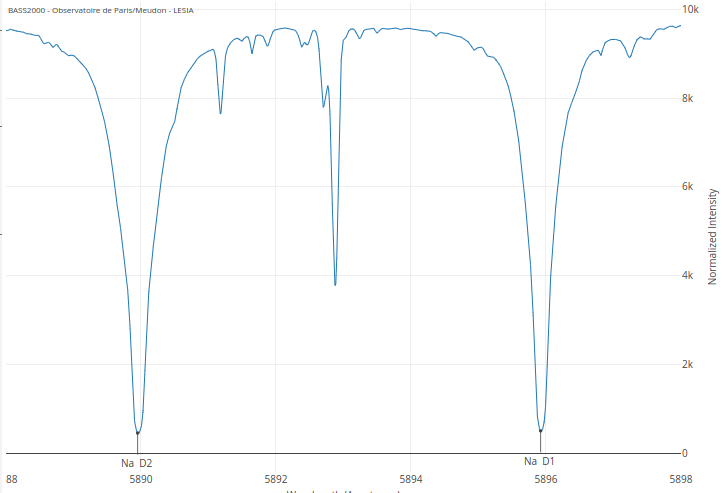
\includegraphics[width=6.5cm]{figures/naD.png}
\caption{Spectral lines of neutral Sodium (Na). Credits: Observatoire de Paris/Meudon}
\end{figure}
\end{minipage}

}
%
%
\frame{
\frametitle{Ok maybe one more slide}
\begin{minipage}{0.55\textwidth}
\begin{itemize}
\item If we can ``tune'' to specific wavelengths in a spectral line, this allows us to observe specific heights in the atmosphere.
\item \q{Discuss that, with the help of the blackboard if needed.}
\item Spectral lines are also important because they are sensitive to velocities and magnetic fields. 
\item A bit more about this in the next lecture (we talk about the Sun).
\item And much more about this in the next semester: Experimental Astrophysics I: Remote Sensing.
\item See you Friday for a numerical exercise!
\end{itemize}
\end{minipage}
\begin{minipage}{0.44\linewidth}
\begin{figure}
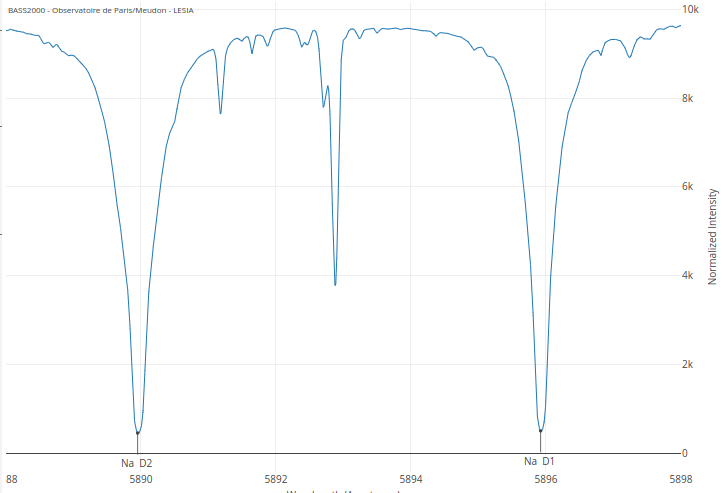
\includegraphics[width=6.5cm]{figures/naD.png}
\caption{Spectral lines of neutral Sodium (Na). Credits: Observatoire de Paris/Meudon}
\end{figure}
\end{minipage}

}
%

\end{document}
% 

